%
% teil2.tex -- Beispiel-File für teil2 
%
% (c) 2020 Prof Dr Andreas Müller, Hochschule Rapperswil
%
% !TEX root = ../../buch.tex
% !TEX encoding = UTF-8
%
\section{Einfacher Bruteforce Algorithmus}
In der Bruteforce Methode wird jede Variante durchprobiert, 
um die beste Lösung zu finden. Dabei wird Systematisch ein 
Ablauf durchgemacht und überprüft, wie lange die Strecke ist.
Ist die Strecke kürzer ist dies die neue Optimale Lösung.

\begin{figure} [h]
	\centering
	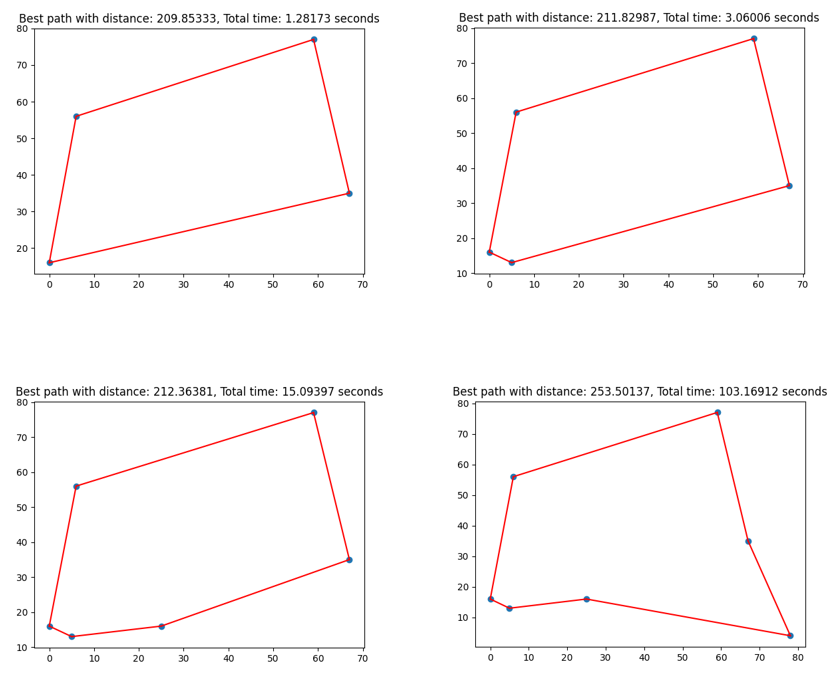
\includegraphics[width=0.8\textwidth]{
        papers/variationsprinzip_algorithmen/images/teil2/02_bruteforce_methode.jpg
        }
	\caption{Abbildung Verschiedener Durchgänge mit steigender Anzahl von Städten}
	\label{fig:Abbildung Verschiedener Durchgänge mit steigender Anzahl von Städten}
\end{figure}

Auf dem Bild ist ersichtlich das mit jedem weiteren Knoten der Aufwand 
exponentiell steigt oder anders ausgedrückt, mit jeder weiteren Knoten
gibt es mehr Variationen, die durchprobiert werden müssen. Dies lässt
sich mit der Formel

\begin{equation}
    (n-1)!
\end{equation}

berechnen. Dabei ist \(n\) die Anzahl der Städte.

Der Script lässt sich Mathematisch mit folgender Formel beschreiben:

\begin{equation}
    L(\sigma) = \sum_{i=1}^{n-1} d(\sigma(i), \sigma(i+1)) + d(\sigma(n), \sigma(1))
\end{equation}

